\chapter{Návrh aplikácie}
\label{kap:navrh}

V tejto kapitole uvedieme informácie o architektúre našej aplikácie, návrhu databázy a význam jej tabuliek, spôsob akým budeme údaje od študentov prenášať, zadefinujeme akcie, ktoré vyvolávajú tento prenos a popíšeme fremework Node.js spolu s modulmi, ktoré sme sa rozhodli použiť.

\section{Architektúra toku dát}
\label{sec:architekturadata}

\begin{figure}[h]
	\centerline{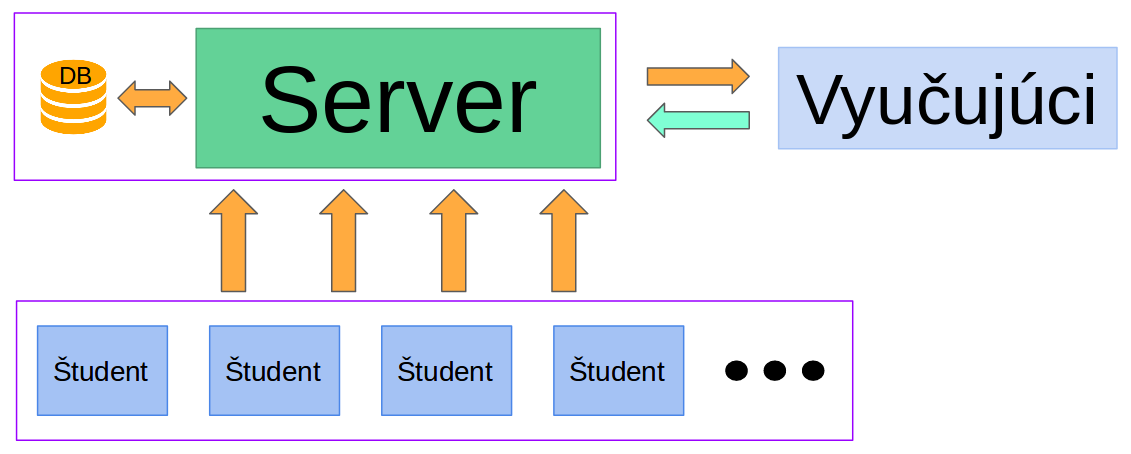
\includegraphics[width=0.9\textwidth]{images/architekturadat.png}}
	\caption[Architektúra toku dát]{Architektúra toku dát.}
	\label{img:architekturadata}
\end{figure}

Obrázok \ref{img:architekturadata} ilustruje tok dát. Každý študent v učebni pracuje
na počítači v Linuxovom termináli. V ňom beží aplikácia GTA, ktorá odosiela dáta
priamo na server šifrované pomocou TLS. Ten ich spracuje, patrične uloží v databáze
a okamžite pošle vyučujúcim, kde sa zobrazia vo webovom rozhraní.

Vyučujúci môžu napríklad vytvárať nové inštancie cvičenia, hodnotiť riešenia študentov.
Dáta v tomto prípade posielame POST požiadavkami na server. Spojenie medzi klientom
a serverom je taktiež šifrované.

\section{Návrh databázy}
\label{sec:navrhdb}

Tabuľky sme navrhli do nasledujúcej štruktúry (viď~\ref{img:navrhdb}).
Väčšina tabuliek sa odkazuje na cudzí kľúč \textit{exercise\_id} z tabuľky
\textit{Exercise}. Tá reprezentuje konkrétnu inštanciu cvičenia. Má nastavený svoj
špecifický identifikátor, meno, posledný level, čas začiatku a konca a stav, v
akom sa nachádza. Možné stavy cvičenia sú \textit{scheduled} (naplánované),
\textit{active} (prebiehajúce), \textit{done} (ukončené).

V tabuľke \textit{Post} sa ukladajú dáta, ktoré posiela GTA aplikácia. Bližšie
informácie o týchto dátach sú zhrnuté v sekcii~\ref{sec:zbieraniedat}.

Do tabuľky \textit{Pointmap} si zapíšeme koľko bodov bude pridelených študentovi
za jednotlivé prejdené levely pri hodnotení. Položka \textit{is\_bonus} nám hovorí,
či tieto body budú pridelené do súčtu k bonusovým alebo nebonusovým. V aplikácii
GTA sa často vyskytuje aj viacero alternatív jedného levelu. Preto položka
\textit{level} môže obsahovať regulárny výraz, ktorý bude vzorom pre viacero
levelov.

Všetkým vyučujúcim sa uloží vytvorený účet do tabuľky \textit{User}.
Heslo sa ukladá do stĺpca \textit{password}. Aby sme skryli heslo pred útočníkom,
je zahašované funkciou \textit{bcrypt} pred uložením do databázy.

V požiadavkách na systém je aj možnosť obodovať jednotlivé riešenia študentov.
Tieto body sa ukladajú do tabuľky \textit{Evaluate}. Pri hodnotení budeme rozlišovať
body za štandardné a body za bonusové úlohy. K hodnoteniu môže vyučujúci pridať aj
komentár, aby študent získal spätnú väzbu k svojmu riešeniu. V tabuľke sa nachádzajú
dva cudzie kľúče. Prvý, \textit{exercise\_id}, odkazuje na cvičenie, v ktorom je študent
hodnotený. Druhý, \textit{user\_id}, odkazuje na vyučujúceho, ktorý hodnotil študenta.

Každý vyučujúci má možnosť si rozmiestniť študentov na plátno. Systém si
pamätá toto rozmiestnenie na základe takzvaného \textit{hostname} počítača,
na ktorom študent pracuje. Toto rozmiestnenie uložíme ako JSON objekt skonvertovaný
do textu v stĺpci \textit{positions} a priradíme konkrétnemu vyučujúcemu.

Tabuľka \textit{Alternative} slúži na nastavenie alternatívneho mena pre študenta.
Keďže niektorí študenti pracujú na vlastných počítačoch, ich používateľské meno
nekorešponduje s menom v systéme Moodle a pri importovaní bodov z csv súboru
by nastala chyba.

\begin{figure}[h]
	\centerline{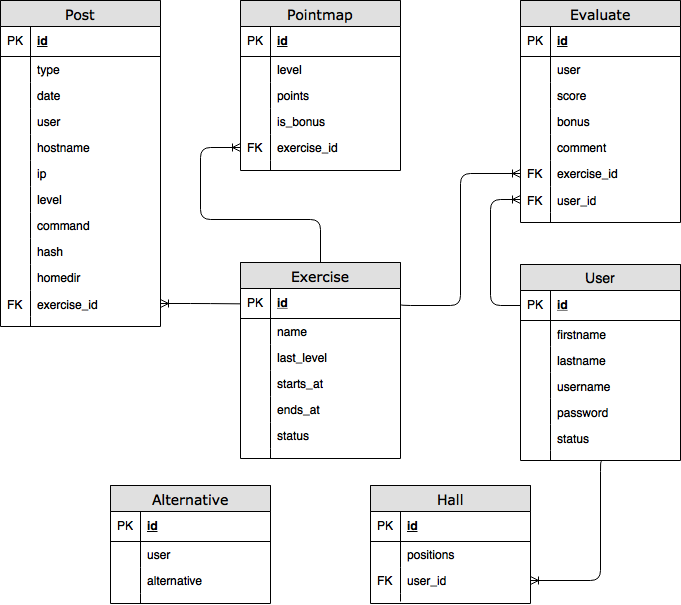
\includegraphics[width=1\textwidth]{images/tabulky.png}}
	\caption[Návrh databázových tabuliek]{Návrh databázových tabuliek a vzťahov medzi nimi.}
	\label{img:navrhdb}
\end{figure}
\clearpage

\section{Zbieranie dát z GTA aplikácie}
\label{sec:zbieraniedat}

Dáta budú na server posielané požiadavkami typu POST v široko používanom JSON
(JavaScript Object Notation) formáte, ktorý ukladá dáta ako \textit{kľúč: hodnota}.
JSON je nezávislý na použití programovacieho jazyka. Pôvodne bol odvodený
z JavaScriptu. Pracuje sa s ním veľmi jednoducho a dáta sú pre človeka ľahko
čitateľné.

Každá požiadavka bude obsahovať nasledujúce základné informácie:

\begin{lstlisting}[language=json,firstnumber=1]
{
    "type": "typ poziadavky",
    "user": "$USER",
    "hostname": "`hostname`",
    "ip": "ip pocitaca",
    "exercise_number": "ID cvicenia",
    "date": "datum a cas"
}
\end{lstlisting}

Špecifikujme ďalej rôzne typy POST požiadaviek. Tie definujú všetky akcie, ktoré
môžu nastať pri riešení úloh.

\subsubsection{Typ \textit{start}}
\label{sec:zbieraniedat:start}

Keď študent spustí GTA skript, systém si poznačí študenta, ktorý začína riešiť cvičenie.

\begin{lstlisting}[language=json,firstnumber=1]
{
    "type": "start",
    "user": "$USER",
    "hostname": "`hostname`",
    "ip": "ip pocitaca",
    "exercise_number": "ID cvicenia",
    "date": "datum a cas"
}
\end{lstlisting}

\subsubsection{Typ \textit{command}}
\label{sec:zbieraniedat:gtadata:command}

Keď študent napíše v termináli príkaz a stlačí enter, odošleme informáciu o príkaze.
Položka \textit{level} označuje level, v ktorom sa študent nachádza. Položka
\textit{command} označuje odoslaný príkaz.

\begin{lstlisting}[language=json,firstnumber=1]
{
    "type": "command",
    "user": "$USER",
    "hostname": "`hostname`",
    "ip": "ip pocitaca",
    "exercise_number": "ID cvicenia",
    "date": "datum a cas",
    "level": "ID levelu",
    "command": "prikaz z terminalu",
}
\end{lstlisting}

\subsubsection{Typ \textit{passed}}
\label{sec:zbieraniedat:gtadata:passed}

Keď študent prejde level, namiesto typu \textit{command} odošleme \textit{passed},
keďže chceme mať záznam o tom, akým príkazom sa študentovi podarilo prejsť daný level.

\begin{lstlisting}[language=json,firstnumber=1]
{
    "type": "passed",
    "user": "$USER",
    "hostname": "`hostname`",
    "ip": "ip pocitaca",
    "exercise_number": "ID cvicenia",
    "date": "datum a cas",
    "level": "ID levelu",
    "command": "prikaz z terminalu",
    "hash": "hash uspesnosti cvicenia",
    "homedir": "$HOME"
}
\end{lstlisting}

\subsubsection{Typ \textit{exit}}
\label{sec:zbieraniedat:exit}

Keď študent ukončí cvičenie napísaním \textit{exit} v termináli,
systém si poznačí, že daný študent skončil a môže zaradiť jeho riešenie
na ohodnotenie.

\begin{lstlisting}[language=json,firstnumber=1]
{
    "type": "exit",
    "user": "$USER",
    "hostname": "`hostname`",
    "ip": "ip pocitaca",
    "exercise_number": "ID cvicenia",
    "date": "datum a cas",
    "hash": "hash uspesnosti cvicenia",
    "homedir": "$HOME"
}
\end{lstlisting}

\subsubsection{Typ \textit{help}}
\label{sec:zbieraniedat:help}

Keď študent potrebuje pomôcť s úlohou, odošle príkaz, ktorý upozorní vyučujúcich.
Záznam sa uloží do databázy %moje oci
 a vyučujúci tak získa prehľad o počte žiadostí
o pomoc v jednotlivých leveloch.

\begin{lstlisting}[language=json,firstnumber=1]
{
    "type": "help",
    "user": "$USER",
    "hostname": "`hostname`",
    "ip": "ip pocitaca",
    "exercise_number": "ID cvicenia",
    "date": "datum a cas",
    "level": "ID levelu"
}
\end{lstlisting}

\subsubsection{Typ \textit{ack}}
\label{sec:zbieraniedat:ack}

Po úspešnej pomoci študentovi odošle vyučujúci alebo študent túto informáciu
do našej aplikácie a vytvorí sa záznam v databáze.

\begin{lstlisting}[language=json,firstnumber=1]
{
    "type": "ack",
    "user": "$USER",
    "hostname": "`hostname`",
    "ip": "ip pocitaca",
    "exercise_number": "ID cvicenia",
    "date": "datum a cas",
    "level": "ID levelu"
}
\end{lstlisting}

\section{Node.js}
\label{sec:nodejs}

Node.js je multiplatformový open-source softvér, ktorý spúšťa JavaScriptový
kód na strane servera. Je primárne určený na programovanie webových serverov.
Historicky sa JavaScript používal ako skriptovací jazyk
na strane klienta, kde tento skript bol vložený v HTML stránke a prehliadač ho vedel
stiahnuť a spustiť. Keďže Node.js ponúka vývojárom spúšťanie skriptov na strane servera,
otvára sa možnosť na dynamického generovania stránok predtým, ako sú odoslané do
prehliadača. Ďalej utilizuje takzvanú \glqq JavaScript všade\grqq~paradigmu, ktorá
hovorí o tom, že kód webových aplikácií na strane servera a na strane klienta nepoužíva rozdielne programovacie jazyky.~\cite{bib:nodejs}

Prvýkrát bola táto technológia predstavená na konferencii European JSConf v roku 2009.
Jej autor, Ryan Dahl, kritizoval, že majoritná väčšina programovacích jazykov
na strane servera zbytočne čaká na odpoveď vstupno-výstupnej operácie, alebo
výsledku z databázy. Preto cieľom Node.js je poskytnúť neblokujúci a udalosťami
riadený model. Dovoľuje teda zvýšiť priepustnosť aplikácie, ktorá by inak bola omnoho
nižšia.

Node.js sa silno spolieha na využívanie modulov pri vývoji aplikácií. Združuje
ich takzvaný Node Package Manager (NPM). Pri implementácii našej aplikácie sa opierame
o niekoľko z nich. Nižšie si uvedieme podrobnejšie informácie o týchto moduloch. \cite{bib:crawford2017comparison}

\subsection{Express.js}
\label{sec:nodejs:expressjs}

Express.js je jeden z najpoužívanejších frameworkov pre Node.js. Jeho flexibilnosť
a minimalizmus ponúkajú pohodlný a rýchly vývoj webových aplikácií.
Veľa vylepšení je dostupných v podobe pluginov, ktoré si môžeme nainštalovať z NPM
databázy. My využijeme architektúru \textit{model-view-controller} (MVC). Najskôr príde
požiadavka na server, ktorú obsluhuje \textit{controller}. Pri obsluhovaní
interaguje s databázovým \textit{modelom}. Následne sa zavolá \textit{view}, ktorý 
vyrenderuje stránku a tá sa odošle klientovi do prehliadača. Na renderovanie
stránky využijeme view engine \textit{Pug}, ktorý má plnú podporu pre Express.js
aplikácie.

\subsection{Sequelize}
\label{sec:nodejs:sequelize}

Aby sme vedeli ukladať a manipulovať dáta v databáze, potrebujeme modul \textit{mysql2}.
Avšak, všetky dotazy do databázy treba písať v jazyku sql, čo môže vytvoriť nemalé
množstvo chýb a zneprehľadniť kód.

Objektovo relačné zobrazenie (ORM) je technika
softvérového inžinierstva, ktorá umožňuje automaticky
konvertovať dáta medzi databázou a objektovo orientovaným programovacím jazykom.
~\cite{bib:orm}

Sequelize je ORM modul pre Node.js aplikácie. Podporuje relačné databázy \textit{MySQL},
\textit{MariaDB}, \textit{SQLite}, \textit{PostgreSQL} a \textit{MsSQL}.
Vďaka prehľadnej dokumentácii~\cite{bib:sequelizedocs}, dobrej funkcionalite a veľkej
komunite sme sa rozhodli použiť Sequelize v našej aplikácii.

\subsection{WebSocket a Socket.io}
\label{sec:nodejs:socketio}

WebSocket~\cite{bib:fette2011websocket} je komunikačný protokol, ktorý poskytuje full-duplex asynchrónnu komunikáciu cez
jediné TCP spojenie. Využíva \textit{ws} (nezabezpečený) alebo \textit{wss} (bezpečný)
protokol. Nie je limitovaný ako napríklad AJAX, kde klient musí najskôr vytvoriť
požiadavku na server. Server aj klient si môžu posielať správy jeden druhému bez
obmedzenia. Problém s WebSocketom je, že niektoré staršie prehliadače ho nepodporujú.
Ďalší problém sú firewally, z ktorých väčšina môže blokovať komunikáciu a neumožní
WebSocketu vytvoriť spojenie. Ak by sme sa teda rozhodli použiť čisto WebSocket
protokol, musíme rátať s tým, že naša aplikácia nemusí fungovať správne na všetkých
zariadeniach. Modul Socket.io rieši tento problém. Zariadenia, ktoré
podporujú WebSocket budú fungovať naďalej bez zmeny a pre tie, ktoré ho
nepodporujú, sa Socket.io bude snažiť nájsť najlepšiu možnú alternatívu v
nasledujúcom poradí:
\begin{enumerate}
	\item WebSocket
	\item FlashSocket
	\item XHR long polling
	\item XHR multipart streaming
	\item XHR polling
	\item JSONP polling
	\item iframe
\end{enumerate}

Máme teda zaručené, že aplikácia bude fungovať aj v starších prehliadačoch. Socket.io
poskytuje aj API pre Node.js, ktoré vyzerá a používa sa takmer identicky ako na strane
klienta.~\cite{bib:raisocketio,bib:walshwebsocket}

\subsection{Passport.js}
\label{sec:nodejs:passportjs}

V našej aplikácii potrebujeme autentizovať užívateľov. Prístup do webového
rozhrania aplikácie môže mať len vyučujúci. Passport.js je vhodným modulom
do Node.js aplikácií dobre integrovateľný s Express.js frameworkom.
Podporuje viacero metód autentizácie, napríklad aj OAuth2, Auth0...
My pre jednoduchosť využijeme štandardný prístup pomocou mena a hesla.
Kvalitná dokumentácia~\cite{bib:passportjsdocs} tohto modulu nám pomohla pri
implementácii.